\let\negmedspace\undefined
\let\negthickspace\undefined
\documentclass[journal]{IEEEtran}
\usepackage[a5paper, margin=10mm, onecolumn]{geometry}
%\usepackage{lmodern} % Ensure lmodern is loaded for pdflatex
\usepackage{tfrupee} % Include tfrupee package

\setlength{\headheight}{1cm} % Set the height of the header box
\setlength{\headsep}{0mm}     % Set the distance between the header box and the top of the text

\usepackage{gvv-book}
\usepackage{gvv}
\usepackage{cite}
\usepackage{amsmath,amssymb,amsfonts,amsthm}
\usepackage{algorithmic}
\usepackage{graphicx}
\usepackage{textcomp}
\usepackage{xcolor}
\usepackage{txfonts}
\usepackage{listings}
\usepackage{enumitem}
\usepackage{mathtools}
\usepackage{gensymb}
\usepackage{comment}
\usepackage[breaklinks=true]{hyperref}
\usepackage{tkz-euclide} 
\usepackage{listings}
% \usepackage{gvv}                                        
\def\inputGnumericTable{}                                 
\usepackage[latin1]{inputenc}                                
\usepackage{color}                                            
\usepackage{array}                                            
\usepackage{longtable}                                       
\usepackage{calc}                                             
\usepackage{multirow}                                         
\usepackage{hhline}                                           
\usepackage{ifthen}                                           
\usepackage{lscape}
\begin{document}

\bibliographystyle{IEEEtran}
\vspace{3cm}
\title{12.8.3.18}
\author{EE24BTECH11025 - GEEDI HARSHA}
% \maketitle
% \newpage
{\let\newpage\relax\maketitle}

\renewcommand{\thefigure}{\theenumi}
\renewcommand{\thetable}{\theenumi}
\setlength{\intextsep}{10pt} % Space between text and floats


\numberwithin{equation}{enumi}
\numberwithin{figure}{enumi}
\renewcommand{\thetable}{\theenumi}

\textbf{Question:}
The area of the circle \(x^2 + y^2 = 16\) exterior to the parabola \(y^2 = 6x\) is:


\solution

The circle is given by:
\begin{align*}
x^2 + y^2 &= 16 \quad \Rightarrow \quad r = 4
\end{align*}

The parabola is given by:
\begin{align*}
y^2 &= 6x
\end{align*}
\subsection*{Parabola Equation}
\[
g\brak{\vec{x}} = \vec{x}^\top \vec{V_1} \vec{x} + 2 \vec{u_1}^\top \vec{x} + f_1 = 0,
\]
\subsection*{Circle Equation}
\[
g\brak{\vec{x}} = \vec{x}^\top \vec{V_2} \vec{x} + 2 \vec{u_2}^\top \vec{x} + f_2 = 0,
\]
\begin{itemize}
    \item \( \mu = -\frac{4}{9} \)
    \item \( V_1 = \begin{pmatrix} 0 & 0 \\ 0 & 1 \end{pmatrix} \)
    \item \( V_2 = \begin{pmatrix} \frac{9}{4} & 0 \\ 0 & \frac{9}{4} \end{pmatrix} \)
    \item \( f_1 = 0 \)
    \item \( f_2 = -\frac{81}{16} \)
    \item \( u_1 = \begin{pmatrix} -2 \\ 0 \end{pmatrix} \)
    \item \( u_2 = \begin{pmatrix} 0 \\ 0 \end{pmatrix} \)
\end{itemize}

\textbf{Step 1: Matrix \( V_1 + \mu V_2 \):}
\[
V_1 + \mu V_2 = \begin{pmatrix} 0 & 0 \\ 0 & 1 \end{pmatrix} + \left(-\frac{4}{9}\right) \begin{pmatrix} \frac{9}{4} & 0 \\ 0 & \frac{9}{4} \end{pmatrix} = \begin{pmatrix} -1 & 0 \\ 0 & 0 \end{pmatrix}.
\]

\textbf{Step 2: Vector \( u_1 + \mu u_2 \):}
\[
u_1 + \mu u_2 = \begin{pmatrix} -2 \\ 0 \end{pmatrix} + \left(-\frac{4}{9}\right) \begin{pmatrix} 0 \\ 0 \end{pmatrix} = \begin{pmatrix} -2 \\ 0 \end{pmatrix}.
\]

\textbf{Step 3: Scalar \( f_1 + \mu f_2 \):}
\[
f_1 + \mu f_2 = 0 + \left(-\frac{4}{9}\right)(-16) = \frac{64}{9}.
\]

\textbf{Step 4: Combined Equation:}
\[
\vec{x}^\top (V_1 + \mu V_2) \vec{x} + 2 (u_1 + \mu u_2)^\top \vec{x} + (f_1 + \mu f_2) = 0,
\]
\[
\begin{pmatrix} x \\ y \end{pmatrix}^\top \begin{pmatrix} -1 & 0 \\ 0 & 0 \end{pmatrix} \begin{pmatrix} x \\ y \end{pmatrix} + 2 \begin{pmatrix} -2 \\ 0 \end{pmatrix}^\top \begin{pmatrix} x \\ y \end{pmatrix} + \frac{64}{9} = 0.
\]

Expanding the terms:
\[
-\frac{4}{9}x^2 + \frac{5}{9}y^2 - 6x + \frac{64}{9} = 0.
\]

Multiplying through by 9:
\[
-4x^2 + 5y^2 - 54x + 64 = 0.
\]

\textbf{Substitute \( y^2 = 6x \) into the equation:}
\[
-4x^2 + 5(6x) - 54x + 64 = 0,
\]
\[
-4x^2 + 30x - 54x + 64 = 0,
\]
\[
-4x^2 - 24x + 64 = 0.
\]

Dividing through by -4:
\[
x^2 + 6x - 16 = 0.
\]

Solving using the quadratic formula:
\[
x = \frac{-6 \pm \sqrt{6^2 - 4(1)(-16)}}{2(1)} = \frac{-6 \pm \sqrt{36 + 64}}{2} = \frac{-6 \pm \sqrt{100}}{2}.
\]

\[
x = \frac{-6 \pm 10}{2}.
\]

Thus, the solutions for \( x \) are:
\[
x = 2 \quad \text{or} \quad x = -8.
\]

\textbf{For \( x = 2 \), solve for \( y \):}
\[
y^2 = 6x = 12 \implies y = \pm \sqrt{12} = \pm 2\sqrt{3}.
\]

\textbf{For \( x = -8 \), the equation \( y^2 = -48 \) has no real solutions.}

Thus, the intersection points are:
\[
(2, 2\sqrt{3}) \quad \text{and} \quad (2, -2\sqrt{3}).
\]
The area outside the parabola and inside the circle is given by:
\begin{align*}
\text{Area} &= \text{Total Circle Area} - 2 \times \int_0^2 \sqrt{6x} \, dx
\end{align*}

1. Total circle area:
\begin{align*}
A_{\text{circle}} &= \pi r^2 = 16\pi
\end{align*}

2. Area under the parabola:
\begin{align*}
\int_0^2 \sqrt{6x} \, dx &= \int_0^2 \sqrt{6} \sqrt{x} \, dx = \sqrt{6} \int_0^2 x^{1/2} \, dx \\
&= \sqrt{6} \left[\frac{2}{3}x^{3/2}\right]_0^2 \\
&= \sqrt{6} \cdot \frac{2}{3} \cdot (2^{3/2}) = \frac{4\sqrt{6}}{3}
\end{align*}

Thus, the area outside the parabola is:
\begin{align*}
\text{Area} &= 16\pi - \frac{8\sqrt{6}}{3} \\
&= \quad \frac{4}{3}(4\pi - \sqrt{3})
\end{align*}




\textbf{Computational Solution}\\

The \textbf{Trapezoidal} rule for approximating the integral of a function \(f(x)\) from \(a\) to \(b\) is given by:

\begin{align*}
\int_a^b f(x) \, dx &\approx \frac{h}{2} \left[ f(a) + 2 \sum_{i=1}^{n-1} f(x_i) + f(b) \right]
\end{align*}
where \(h = \frac{b - a}{n}\) is the width of each subinterval\\
 \(x_i = a + ih\) for \(i = 1, 2, \dots, n-1\).\\
$\textbf{Difference equation}$,
\begin{align}
    A_n &= \frac{h}{2}\brak{y\brak{x_0} + y\brak{x_1}} + \frac{h}{2}\brak{y\brak{x_1} + y\brak{x_2}} + \dots + \frac{h}{2}\brak{y\brak{x_{n - 1}} + y\brak{x_{n}}}\\
    A_n &= h\brak{\frac{y\brak{x_0}}{2} + y\brak{x_1} + y\brak{x_2} \dots \frac{y\brak{x_n}}{2}}\\
    A_{n + 1} &= A_n + \frac{h}{2}\brak{y\brak{x_{n + 1}} + y\brak{x_n}} \text{, } x_{n + 1} = x_n + h\\
    A_{n + 1} &= A_n + \frac{h}{2}\brak{y\brak{x_n + h} + y\brak{x_n}}\\
\end{align}
By the first principle of derivative,
\begin{align}
    y^{\prime}\brak{x} &= \lim_{h\to0} \frac{y\brak{x + h} - y\brak{x}}{h}\\
    y\brak{x + h} &= y\brak{x} + h\brak{y^{\prime}\brak{x}} \text{, } h\to0
\end{align}
Rewriting the difference equation, we get,
\begin{align}
    A_{n + 1} &= A_n + \frac{h}{2}\brak{y\brak{x_n} + hy^{\prime}\brak{x_n} + y\brak{x_n}}\\
    A_{n + 1} &= A_n + h\brak{y\brak{x_n} + \frac{h}{2}y^{\prime}\brak{x_n}}\\
    A_{n + 1} &= A_n + hy\brak{x_n} + \frac{h^2}{2}y^{\prime}\brak{x_n}
\end{align}\\
In this case, \(f(x) = \sqrt{6x}\), and we are integrating from \(x = 0\) to \(x = 2\).


We will use \(n = 4\) subintervals for this approximation. Therefore, the width of each subinterval is:

\begin{align*}
h &= \frac{2 - 0}{4} = 0.5
\end{align*}

The points \(x_i\) are:

\begin{align*}
x_0 &= 0, \quad x_1 = 0.5, \quad x_2 = 1, \quad x_3 = 1.5, \quad x_4 = 2
\end{align*}

The corresponding function values are:

\begin{align*}
f(x_0) &= \sqrt{6(0)} = 0, \\
f(x_1) &= \sqrt{6(0.5)} = \sqrt{3}, \\
f(x_2) &= \sqrt{6(1)} = \sqrt{6}, \\
f(x_3) &= \sqrt{6(1.5)} = \sqrt{9} = 3, \\
f(x_4) &= \sqrt{6(2)} = \sqrt{12} = 2\sqrt{3}
\end{align*}

Now, we apply the trapezoidal rule:

\begin{align*}
\int_0^2 \sqrt{6x} \, dx &\approx \frac{0.5}{2} \left[ 0 + 2 \left( \sqrt{3} + \sqrt{6} + 3 \right) + 2\sqrt{3} \right] \\
&= 0.25 \left[ 0 + 2\sqrt{3} + 2\sqrt{6} + 6 + 2\sqrt{3} \right] \\
&= 0.25 \left[ 4\sqrt{3} + 2\sqrt{6} + 6 \right]
\end{align*}
\begin{figure}[h]
    \centering
    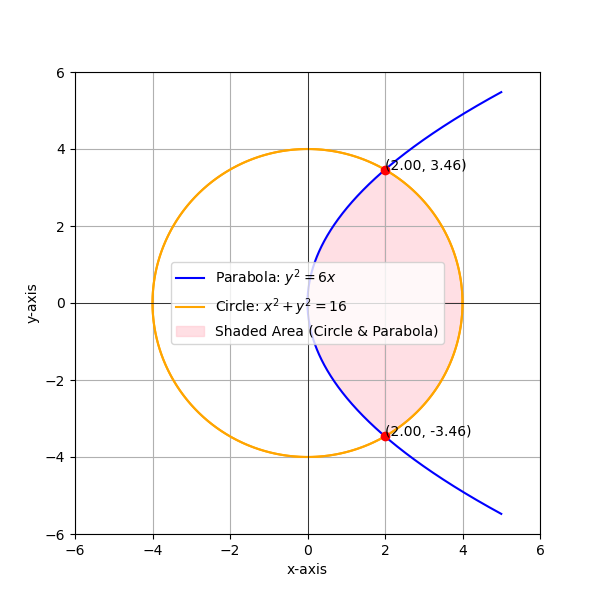
\includegraphics[width=\textwidth]{figs/fig.png}
\end{figure}
\end{document}

